\documentclass{article}
\usepackage[utf8]{inputenc}
\usepackage[english]{babel}
\usepackage[colorinlistoftodos, color=green!40, prependcaption]{todonotes}
\usepackage{amsthm}
\usepackage{mathtools}
\usepackage{physics}
\usepackage{xcolor}
\usepackage{graphicx}
\usepackage[left=23mm,right=13mm,top=35mm,columnsep=15pt]{geometry} 
\usepackage{adjustbox}
\usepackage{placeins}
\usepackage[T1]{fontenc}
\usepackage{lipsum}
\usepackage{gensymb}
\usepackage{siunitx}
\usepackage{float}
\usepackage[
    backend=bibtex, 
    natbib=true,
    style=phys,
    biblabel=brackets,
    giveninits=true,
    abbreviate=false,
    doi=false, url=true, isbn=false,
    block=space,
    backref=true, backrefstyle=two,
]{biblatex}
\addbibresource{refs.bib}
\usepackage{array}
\usepackage{booktabs}
\usepackage{rotating}
\usepackage{csquotes}
\usepackage{url}
\usepackage[pdftitle={Article}, pdfauthor={Author}]{hyperref}
\usepackage{authblk}
\title{A Replication of Millikan's Oil Drop Experiment}
\author{Daniel Speller}
\affil{University of Leeds}
\date{\today}

\begin{document}

\maketitle
\begin{abstract}
    This experiment aimed to determine the known constant $q_e$ and compare it with a reference source to determine its precision and show the quantisation of charge. For this a replication of Millikan's oil drop experiment was used, where charged droplets of oil are suspended by magnets. Equating the magnetic force and gravitational force we can determine a value of $q_e$. Most values of $\frac{q_e}{e}$ were in a relevant proximity to an integer value which is evidence for the idea that charge is quantised and also shows us a high precision in the measured value of $q_e$
\end{abstract}
\section{Introduction}
Millikan's Oil Drop experiment is a method of measuring the elementary charge of an electron and shows that electric charge is quantised as displayed by the integer multiples of $q_e$ obtained.The current accepted value of $e$ is $1.602 176 634  x 10^{-19} \ \unit C$ \cite{codata}
\\\\
If a charged oil droplet is suspended in air due to a electric field we can equate forces as such
\begin{equation}\label{1}
    F_e=F_g
\end{equation}
\begin{equation}\label{2}
    qE=mg
\end{equation}
For a uniform electric field this yields,
\begin{equation}\label{3}
    q\frac{V}{d}=mg
\end{equation}
As we are unable to measure the mass of a small oil droplet we can replace it with a product of it volume and density,
\begin{equation}\label{4}
    q\frac{V}{d}=\frac{4}{3}\pi r^3\rho g
\end{equation}
For an object moving at terminal velocity through a fluid of viscosity $\eta$ then the force due to gravity will be equal to the drag force as displayed by Stoke's law,
\begin{equation}\label{5}
    F_g=F_d=6\pi \eta rv
\end{equation}
Therefore we can determine $r$ by the equating equations \ref{4} and \ref{5} and rearranging for
\begin{equation}
    r=\sqrt{\frac{9\eta v}{2\rho g}}
\end{equation}
Substituting this back into equation \ref{4} we obtain a final equation for $q_e$,
\begin{equation}
    q_e=\frac{4d}{3V}\pi\left(\frac{9\eta v}{2\rho g}\right)^{\frac{3}{2}} \rho g
\end{equation}
A correction to account for Stoke's Law can be given by the equation \cite{millikan_1913}
\begin{equation}
    q_c=q\left(1+\frac{A}{r}\right)^{\frac{-3}{2}}
\end{equation}

\section{Method}
The experiment is performed by using an atomizer to produce micron-scale charged droplets by making the droplets pass through a charge fine tip to transfer electrons onto the droplet. A uniform magnetic field was created between two circular plates by running a current between them creating a capacitor. The voltage was adjusted to create a uniform magnetic field in which the oil droplets were motionless due to the magnetic force and gravitational force being equal in magnitude. Whilst removing the voltage and starting a stopwatch simultaneously, a time was recorded in which they traversed a predefined distance from which an average velocity could be calculated. This was repeated for a total of ten times in order to obtain bigger integer multiples of $q_e$ and to record multiple cases of each to improve the accuracy of our findings.


\section{Data}
\begin{table}[h]
\centering
\caption{Experimental Constants and Parameters}
\label{tab:constants}
\begin{tabular}{llll}
\toprule
\textbf{Constant} & \textbf{Value} & \textbf{Uncertainty} & \textbf{Units} \\
\midrule
Temperature in Lab & 20.6 & $\pm \ 0.1$ & \unit{\celsius} \\
Air Pressure in Lab & 101.4 & $\pm \ 0.4$ & \unit{\kilo\pascal} \\
Plate separation, $d$ & 0.0058 & $\pm \ 0.00005$ & \unit{\meter} \\
Acceleration due to gravity, $g$ & 9.81 & -- & \unit{\meter\per\second\squared} \\
Air viscosity, $\eta_{\text{air}}$ & $1.50 \times 10^{-5}$ & $0.01\times10^{-5}$ & \unit{\kilo\gram\per\meter\per\second} \\
Density of oil, $\rho_{\text{oil}}$ & 873 & -- & \unit{\kilo\gram\per\meter\cubed} \\
Magnification scale & $\times$2 & -- & -- \\
\bottomrule
\end{tabular}
\end{table}

\begin{table}[h]
\centering
\caption{Experimental Data (Part 1)}
\label{tab:data_part1}
\begin{tabular}{llllllll}
\toprule
\textbf{Index} & \textbf{Voltage (\unit{V})} & \textbf{Distance (\unit{m})} & \textbf{Fall time (\unit{s})} & \textbf{Velocity  (\unit{ms^{-1}})} & \textbf{$\Delta$ V (\unit{ms^{-1}})} & \textbf{r (\unit{m})} & \textbf{$\Delta$ r (\unit{m})}\\
\midrule
1  & 204  & 2.50E-3 & 68.5  & 3.65E-5 & 4.41E-7 & 5.36E-7 & 3.70E-9  \\
2  & 159  & 2.00E-3 & 27    & 7.41E-5 & 1.14E-6 & 7.64E-7 & 6.43E-9 \\
3  & 202  & 2.00E-3 & 69.72 & 2.67E-5 & 4.32E-7 & 4.75E-7 & 3.92E-9  \\
4  & 472  & 2.00E-3 & 79.17 & 2.85E-5 & 3.98E-7 & 4.55E-7 & 3.76E-9 \\
5  & 100  & 2.00E-3 & 76.44 & 2.68E-5 & 3.99E-7 & 4.57E-7 & 3.76E-9 \\
6  & 76   & 2.00E-3 & 80.86 & 1.84E-5 & 2.76E-7 & 3.81E-7 & 3.15E-9 \\
7  & 75   & 2.00E-3 & 91.10 & 2.20E-5 & 3.30E-7 & 4.16E-7 & 3.42E-9 \\
8  & 49   & 2.00E-3 & 82.63 & 2.42E-5 & 3.64E-7 & 4.37E-7 & 3.58E-9 \\
9  & 44   & 2.00E-3 & 121.24 & 1.65E-5 & 2.48E-7 & 3.61E-7 & 2.56E-9 \\
10 & 35   & 2.00E-3 & 97.02 & 2.06E-5 & 3.10E-7 & 4.03E-7 & 3.31E-9 \\
\bottomrule
\end{tabular}
\end{table}

\begin{table}[h]
\centering
\caption{Experimental Data (Part 2)}
\label{tab:data_part2}
\begin{tabular}{llllllllllll}
\toprule
\textbf{Index} & \textbf{q (\unit{C})}  & \textbf{$\Delta$q (\unit{C})} & \textbf{\% uncertainty}\textbf{$\frac{q_c}{e}$} & \textbf{uncertainty} & \textbf{A} & \textbf{B} & \textbf{$\Delta$ B} \\
\midrule
1  & 1.28E-19 & 0.04E-19 & 1.42E-01 & 0.00170162 & 9.04E-19 \\
2  & 5.05E-19 & 3.76E-10 & 1.34E-01 & 315090195  & 3.76E-18 \\
3  & 1.16E-01 & 6.96E-19 & 1.46E-01 & 397283071  & 4.37E-18 \\
4  & 1.16E-01 & 5.26E-19 & 1.47E-01 & 20585184   & 2.94E-18 \\
5  & 1.17E-19 & 1.07E-18 & 1.47E-01 & 80794720   & 1.07E-18 \\
6  & 1.16E-19 & 1.14E-19 & 7.45E-19 & 0.71582729 & 7.45E-19 \\
7  & 1.16E-01 & 1.05E-18 & 1.60E-01 & 0.96381886 & 1.08E-18 \\
8  & 1.16E-01 & 1.15E-18 & 1.48E-01 & 1.60746489 & 2.13E-18 \\
9  & 1.16E-01 & 1.65E-19 & 1.55E-01 & 1.03241457 & 1.06E-18 \\
10 & 2.98E-19 & 1.97E-18 & 1.51E-01 & 1.8618943  & 1.97E-18 \\
\bottomrule
\end{tabular}
\end{table}


\begin{figure}[H]
    \centering
    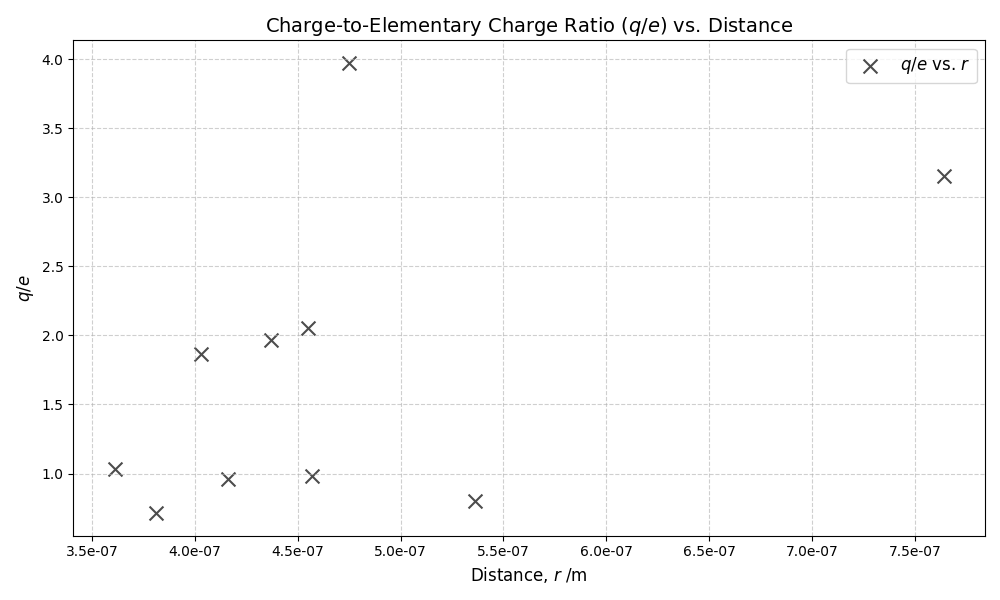
\includegraphics[width=1\linewidth]{Figure_1.png}
    \label{fig:3}
\end{figure}

\section{Analysis}
We can derive our uncertainty for $r$ as follows
\begin{align*}
r &= \sqrt{\frac{9}{2} \frac{\eta_{\text{air}} v}{\rho_{\text{oil}} g}} \\
\ln r &= \frac{1}{2} \ln\left(\frac{9}{2g\rho}\right) + \frac{1}{2} \ln(\eta_{\text{air}}) + \frac{1}{2} \ln(v) \\
\frac{\Delta r}{r} &= \sqrt{
    \left( \frac{1}{2} \frac{\Delta \eta_{\text{air}}}{\eta_{\text{air}}} \right)^2 
    + \left( \frac{1}{2} \frac{\Delta v}{v} \right)^2
} \\
\intertext{Uncertainty in \( v = \frac{x}{t} \)}
\frac{\Delta v}{v} &= \sqrt{
    \left( \frac{\Delta x}{x} \right)^2 
    + \left( \frac{\Delta t}{t} \right)^2
} \\
\Rightarrow \frac{\Delta r}{r} &= \sqrt{
    \left( \frac{1}{2} \frac{\Delta \eta_{\text{air}}}{\eta_{\text{air}}} \right)^2 
    + \frac{1}{4} \left( \left( \frac{\Delta x}{x} \right)^2 + \left( \frac{\Delta t}{t} \right)^2 \right)
}
\end{align*}
For q,
\begin{align*}
q &= \frac{4d}{3V} \pi r^2 \rho_{\text{oil}} g \\
\ln q &= \ln {\frac{4\pi\rho g}{3}} + \ln d + 2 \ln r - \ln V \\
\frac{\Delta q}{q} &= \sqrt{
    \left( \frac{\Delta d}{d} \right)^2 
    + \left( \frac{2 \Delta r}{r} \right)^2 
    + \left( \frac{\Delta V}{V} \right)^2
} \\
\intertext{{With correction \( q_c = q \cdot B^{-3/2} \)}:}
\frac{\Delta q_c}{q_c} &= \sqrt{
    \left( \frac{\Delta q}{q} \right)^2 
    + \left( \frac{3 A \Delta r}{2 r (r + A)} \right)^2
} \\
&= \sqrt{
    \left( \frac{\Delta d}{d} \right)^2 
    + \left( \frac{2 \Delta r}{r} \right)^2 
    + \left( \frac{\Delta V}{V} \right)^2
    + \left( \frac{3 A \Delta r}{2 r (r + A)} \right)^2
}
\end{align*}
For comparing elementary charge to corrected values of $q_c$, the uncertainty is simply
\begin{align*}
\Delta \left(\frac{q_c}{e}\right)=\frac{\Delta q_c}{e}
\end{align*}
\section{Discussion}
The major source of error in this experiment is the uncertainty that comes from the time being measured manually, as even a small uncertainty of $\pm 0.1$ \unit{s} could lead to a significantly greater uncertainty of $q_e$. Another potential source of systematic error in this experiment is the change in viscosity of the oil as it is a temperature dependent value and would fluctuate in accordance with changes of temperature in the lab. $2$ accurate average values of $\frac{q_e}{e}$  were found at $n=1$ and $n=2$ quantisation level as these has at least 3 values to average. These were calculated to be $0.898$ and $1.96$  respectively representing a $10.2\%$ and $4\%$ difference to the expected value of $1$ and $2$   
\section{Conclusion}
Overall, this experiment was a success with all but one calculated $q/e$ value  being close to an integer. If the experiment were to be performed again it would be beneficial to increase the amount of droplets analysed as well as introducing a systematic approach to analyse multiple droplets of the same size.


\printbibliography

\end{document}
